\section{Introduzione}
Il presente progetto, per il corso di \textit{Big Data}, propone un sistema di monitoraggio dei dati provenienti da sensori installati in un noccioleto nel contesto del progetto \textit{PANTHEON}.\par

\subsection{Progetto PANTHEON}
PANTHEON è un progetto finanziato dall'Unione Europea nel contesto del programma H2020 che si pone come obiettivo quello di realizzare l'equivalente di un sistema industriale di \textit{Supervisory Control And Data Acquisition (SCADA)} nel contesto dell'\textit{agricoltura di precisione}.\par

In particolare l'obiettivo di PANTHEON è quello di progettare un sistema per la gestione dei noccioleti composto da una serie di elementi robotici (sia terresti che aerei) che si muovono all'interno della coltura di interesse e una rete di sensori IoT, alimentati ad energia solare, per monitorare costantemente le condizioni ambientali della coltura in cui sono installati.\par

Le informazioni raccolte dai robot e dai sensori vengono poi collezionate in una unità operativa centrale che analizza i dati per poter poi eseguire automaticamente opportune azioni (come ad esempio avviare il sistema di irrigazione) oltre a supportare le decisioni degli agronomi relativamente alla gestione del noccioleto.\par

In particolare il sistema proposto in PANTHEON prevede di raccogliere dati relativi alle singole piante al fine di monitorare meglio le condizioni complessive della coltura oltre a migliorare l'efficacia e l'efficienza delle operazioni agricole tipicamente effettuate.\par

Ad esempio, nel contesto dell'irrigazione si può pensare di irrigare un particolare gruppo di piante che hanno particolare necessità di acqua piuttosto che l'intera coltivazione, portando a dei risparmi in termini di quantità d'acqua impiegata per l'irrigazione. Analogo discorso può essere esteso all'applicazione dei pesticidi.\par

\begin{figure}[ht]
\centering
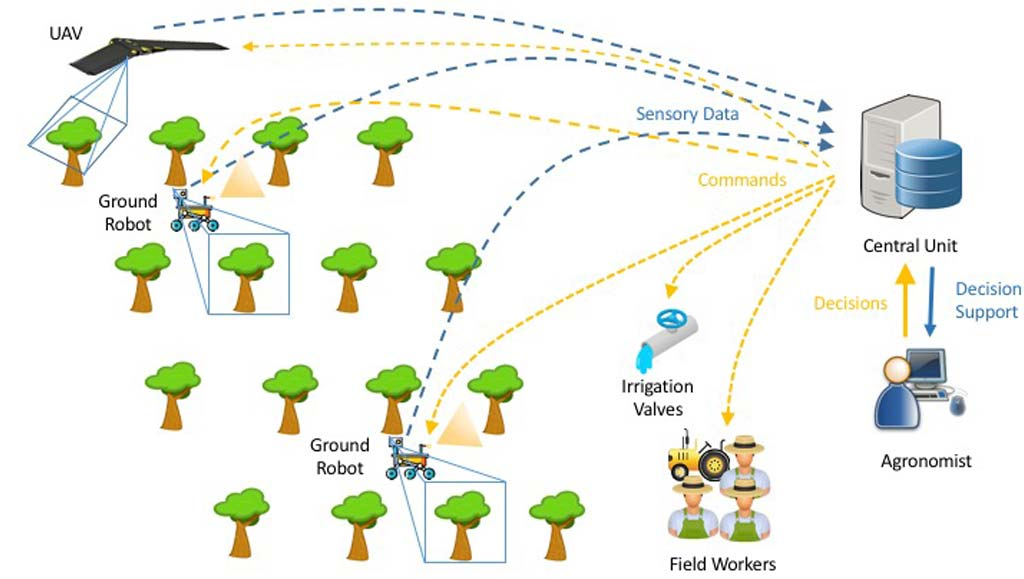
\includegraphics[width=1\textwidth]{vision}
\caption{Panoramica del progetto PANTHEON}
\label{fig:vision}
\end{figure}

\subsubsection{Architettura software del progetto PANTHEON} \label{pantheon-architecture}
Al fine di gestire l'enorme mole di dati in tempo reale provenienti dai sensori e dai robot, gli autori del progetto PANTHEON hanno ideato una architettura software composta da tecnologie pensate per gestire e manipolare \textit{big data}, come l'ecosistema \textit{Hadoop} e i sistemi \textit{noSQL}.\par

In particolare l'architettura si compone fondamentalmente di tre blocchi (si vedano anche le figure \ref{fig:architecture1} e \ref{fig:architecture2}):
\begin{itemize}
  \item \textit{Data Collection e Pre-processing layer (DCP layer)}, che è uno strato che viene replicato per ogni noccioleto e si occupa della collezione dei dati provenienti dai sensori e dai robot presenti nell'appezzamento di terreno in questione.  
  \item \textit{Data Transfer layer (DT layer)}, che è uno strato di middleware che si occupa di consentire il trasferimento di dati tra il DCP layer e il DSP layer (descritto di seguito) in entrambe le direzioni anche in assenza di connessione di rete.
  \item \textit{Data Storage and Processing layer (DSP layer)}, che consiste in una unità centrale in cui confluiscono i dati provenienti dai vari layer DCP delle varie colture. Tali dati vengono memorizzati e analizzati secondo un approccio \textit{data lake}, dove viene impiegato una grande \textit{repository} centrale per poter memorizzare e processare dati (anche eterogenei) provenienti dalle varie sorgenti.
\end{itemize}

\begin{figure}[ht]
\centering
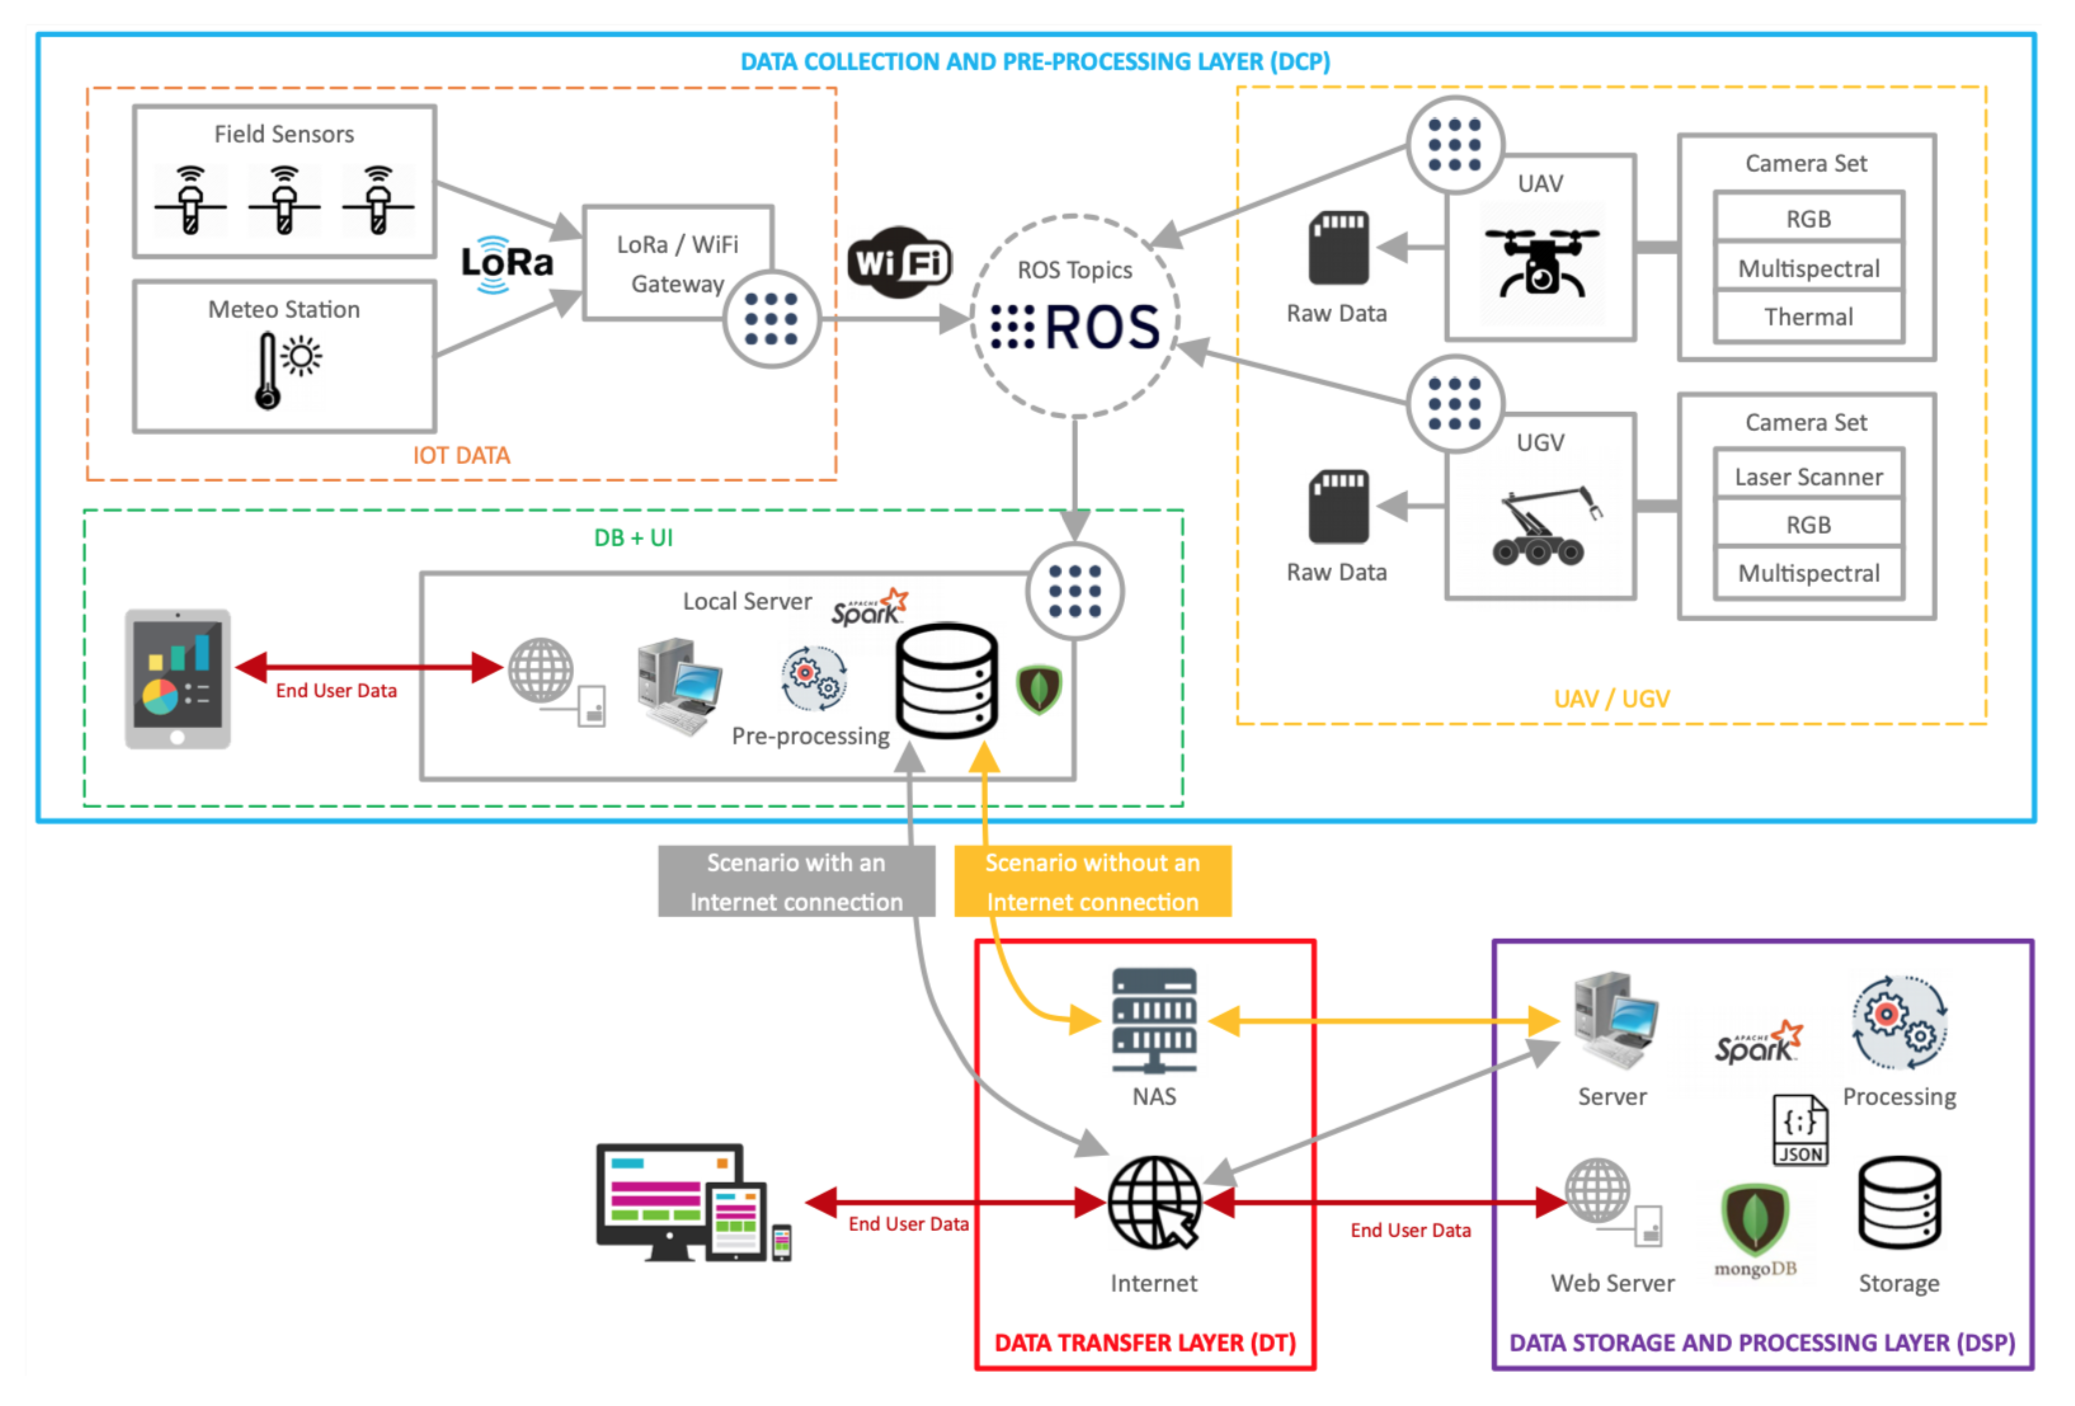
\includegraphics[width=1\textwidth]{architecture1}
\caption{Architettura software del progetto PANTHEON}
\label{fig:architecture1}
\end{figure}

\begin{figure}[ht]
\centering
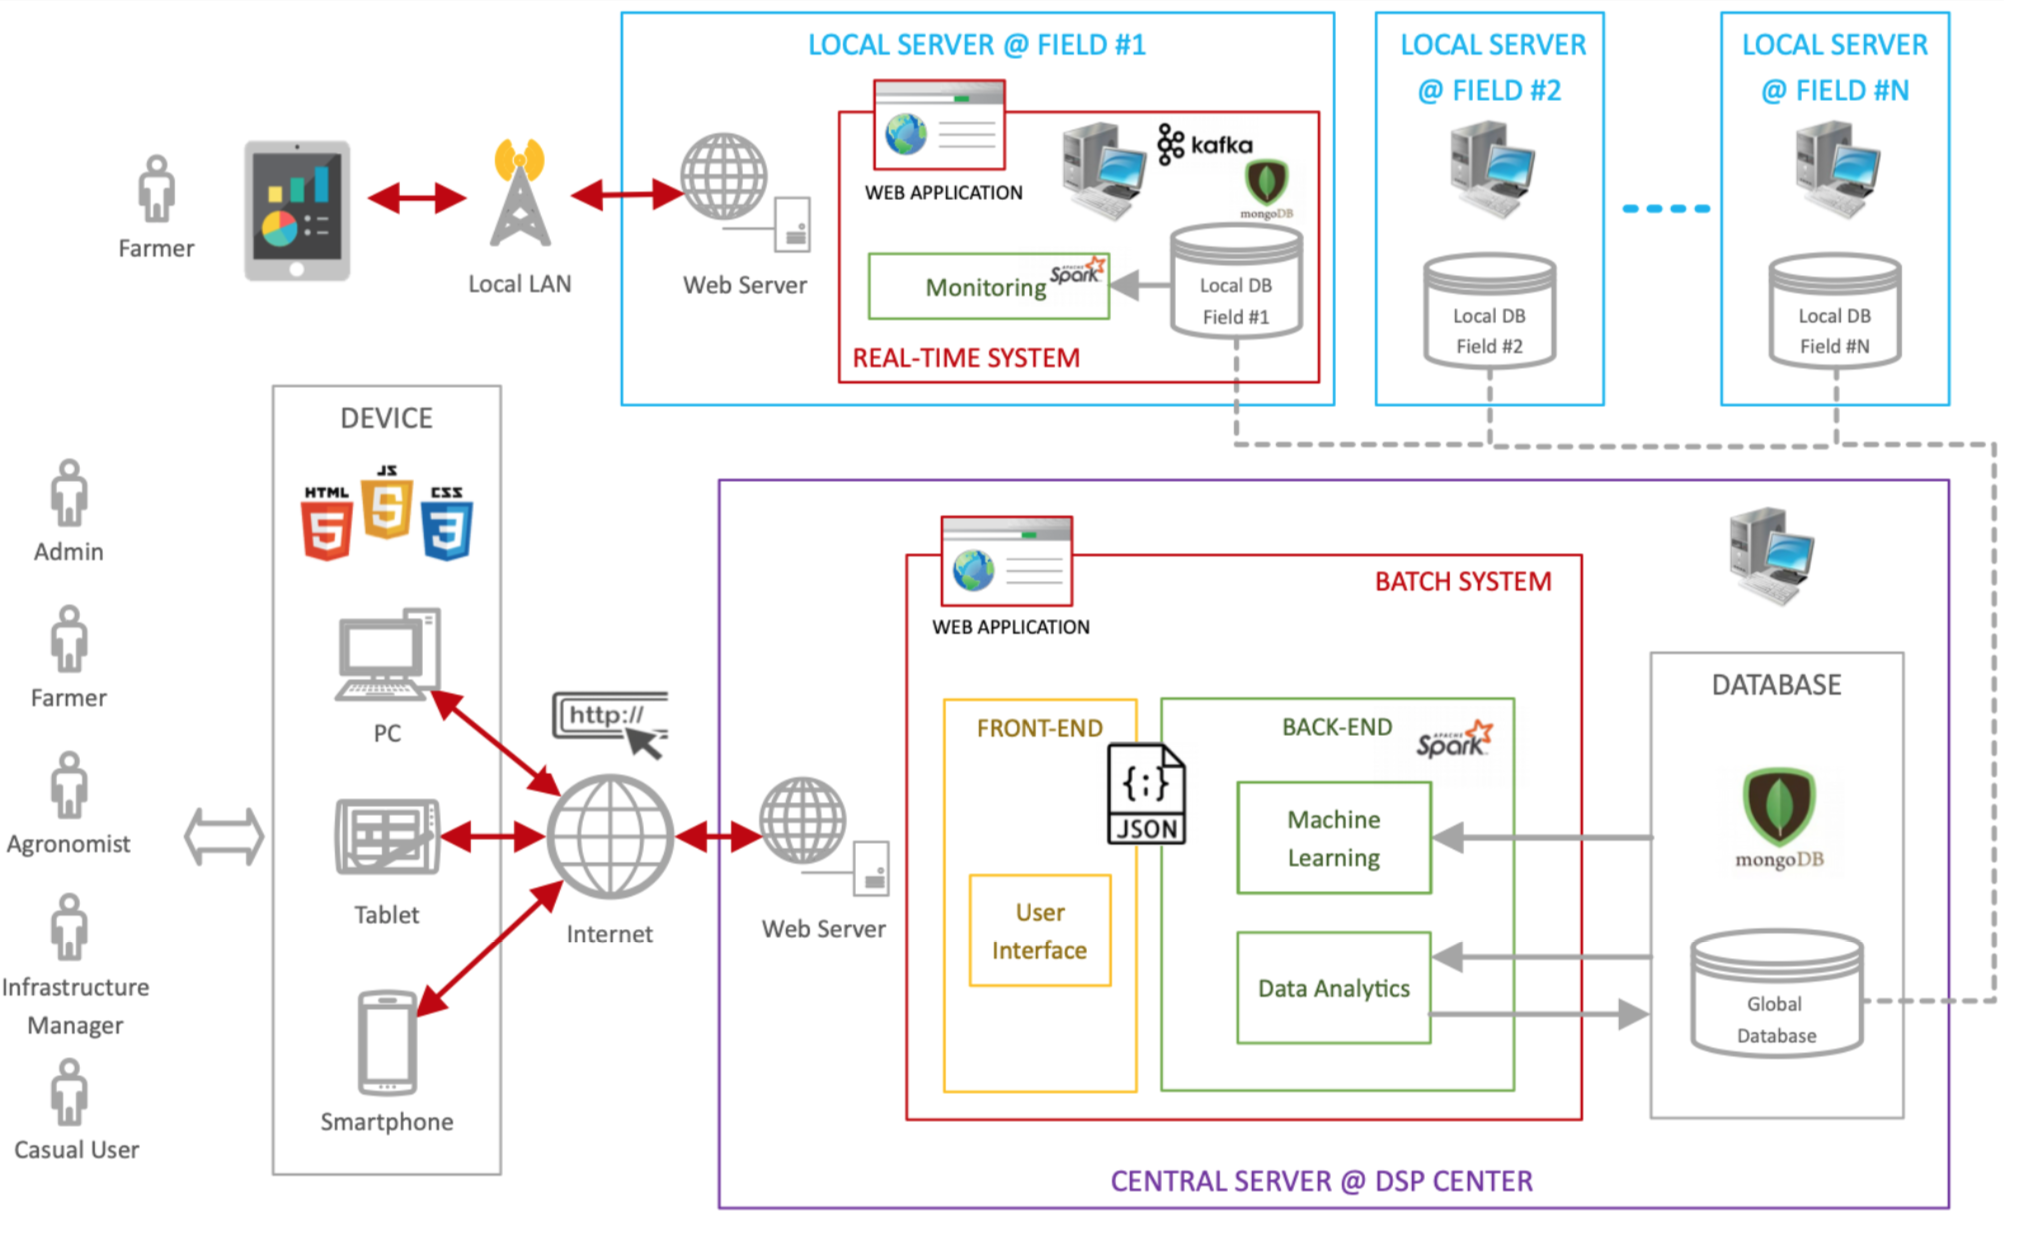
\includegraphics[width=1\textwidth]{architecture2}
\caption{Architettura software del progetto PANTHEON dal punto di vista dell'utente}
\label{fig:architecture2}
\end{figure}